\documentclass[rep.tex]{subfiles}
\begin{document}

\chapter{Zadanie 15}
\label{zad15}
\section{Treść}
Zaprojektować dzielnik sygnału mikrofalowego typu Gysel’a przyjmując $f_0 = 1.35~GHz$ i $Z_0 = 50~\Omega$.
Projekt dzielnika wykonać przy założeniu, że jest on realizowany z odcinków powietrznej,
symetrycznej linii paskowej o grubości $b = 8~mm$.
Grubość przewodu wewnętrznego $t = 0.8~mm$.
Obliczyć charakterystykę sprzężenia $C(f)[dB]$ w paśmie od $f_1 = 1.25~GHz$ do $f_2 = 1.45~GHz$.

\begin{figure}[!htbp]
  \centering
  
\includegraphics[width=0.5\linewidth]{fig/zad15/div}
  \caption{Zarys konstrukcyjny projektowanego dzielnika}
  \label{fig:zad15:div}
\end{figure}

\section{Rozwiązanie}
\subsection{Projekt dzielnika}
Projektowany dzielnik jest przedstawiony na rys.~\ref{fig:zad15:div}.
Impedancje poszczególnych sekcji dzielnika opisane są zależnościami:
\begin{align}
  Z_0 &= 50~\Omega \nonumber \\
  Z_1 &= \sqrt{2} * Z_0 &= 70.7106781187~\Omega \\
  Z_3 &= \frac{Z_0}{\sqrt{2}} &= 35.3553390593~\Omega \\
\end{align}

W celu wyznaczenia parametrów realizacji dzielnika za pomocą symetrycznych linii paskowych wykorzystano rozwiązanie zadania~\ref{zad4}.
Otrzymane szerokości przewodów wewnętrznych wynoszą:
\begin{align}
  w_0 &= 8.58657086038~mm \nonumber \\
  w_1 &= 4.65264251488~mm \nonumber \\
  w_3 &= 14.1720836113~mm \nonumber
\end{align}

\subsection{Charakterystyka sprzężenia dzielnika}
W celu wyznaczenia częstotliwościowej charakterystyki sprzężenia:
\begin{align}
  C(f) &= 20 \log \frac{1}{|S_{12}|} \label{eqn:zad15:C} \\
  S_{12} &= \frac{2}{R_{22} + jX_{22}}
\end{align}

\begin{figure}[!htbp]
  \centering
  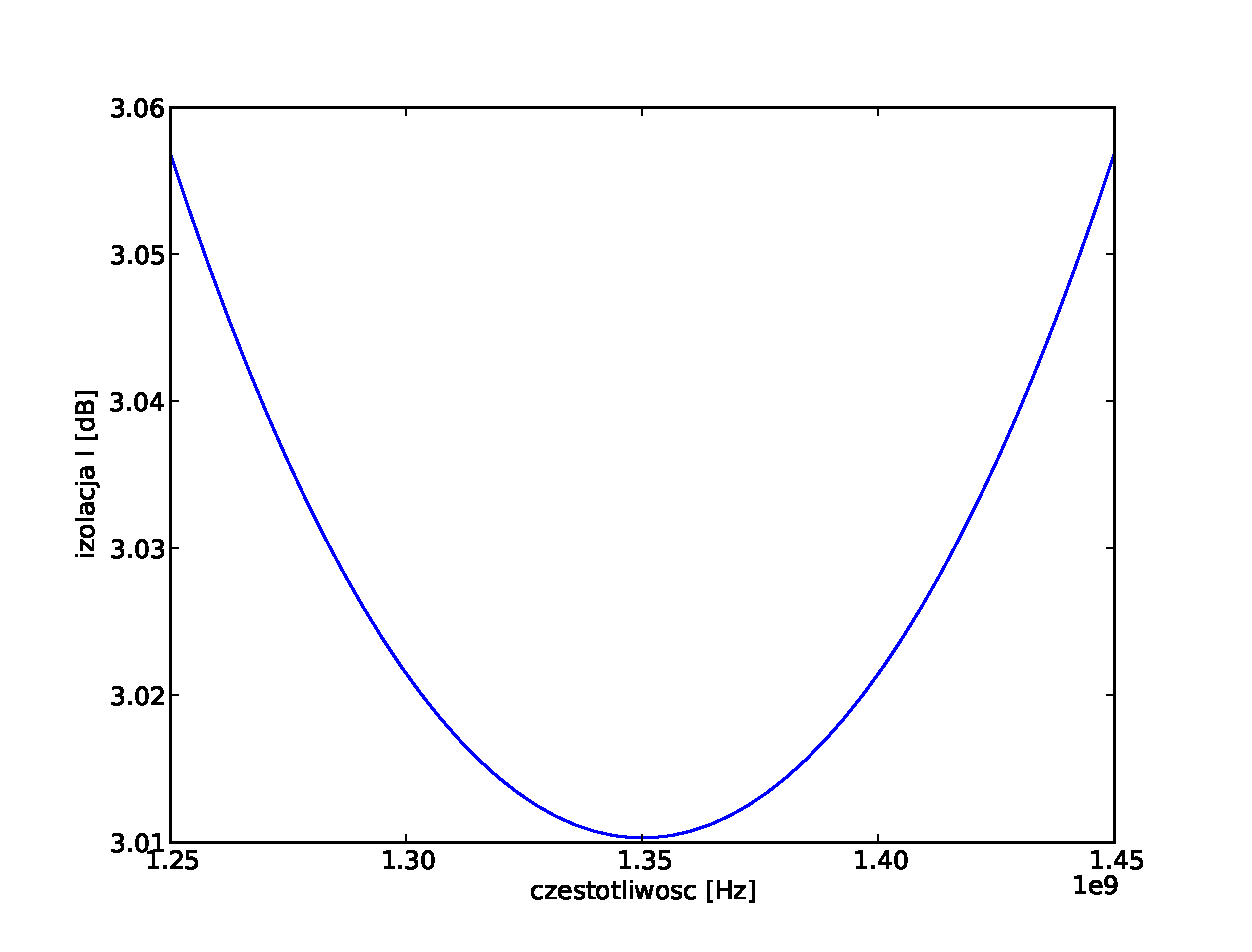
\includegraphics[scale=0.5]{fig/zad15/freq}
  \caption{Charakterystyka sprzężenia dzielnika}
  \label{fig:zad15:freq}
\end{figure}

Dokładne zależności podane zostały w~\cite{obwody}.
Charakterystyki dzielnika zaprezentowano na rys.~\ref{fig:zad15:freq}.
\end{document}
